% Generated by pysimcount.pfchilds -- do not edit; regenerate instead.
% figure: grouping-cnot-twogroup-even-out -- Every formula, two-group grouping (twogroup-even-out), cnot gates vs n (even n only)
% source: ../np-grouping/aggregate.json (seeds [1, 2, 3, 4, 5, 6, 7, 8, 9, 10]); run commits: 01d3c275ceae2840002bd1aaea68f59b987c4975
% metric=cnot kind=twogroup-even-out merged (cz, simcount template)
% measured n: mean over seeds of the run's totals; bars min..max over seeds
% r from power-law fit to mean measured r (n = 6--10); r = ceil(a n^b); point=mean-r-fit; bars = min..max of per-seed fits
% per-step counts exactly affine in n (checked on n = [10, 20, 40], direct build at n = [100])
% shown: suzuki4, suzuki6, mo-q6, mo-q14, bm-q10, mo-o8-q21, morales-y8m10, morales-m8
% removed (see grouping-cnot-twogroup-even-out-ranking.md): lie-trotter, suzuki2, suzuki8
% figure made at git_commit=e5d9ee696f892e28aced765585653760f8a427c4 git_dirty=False
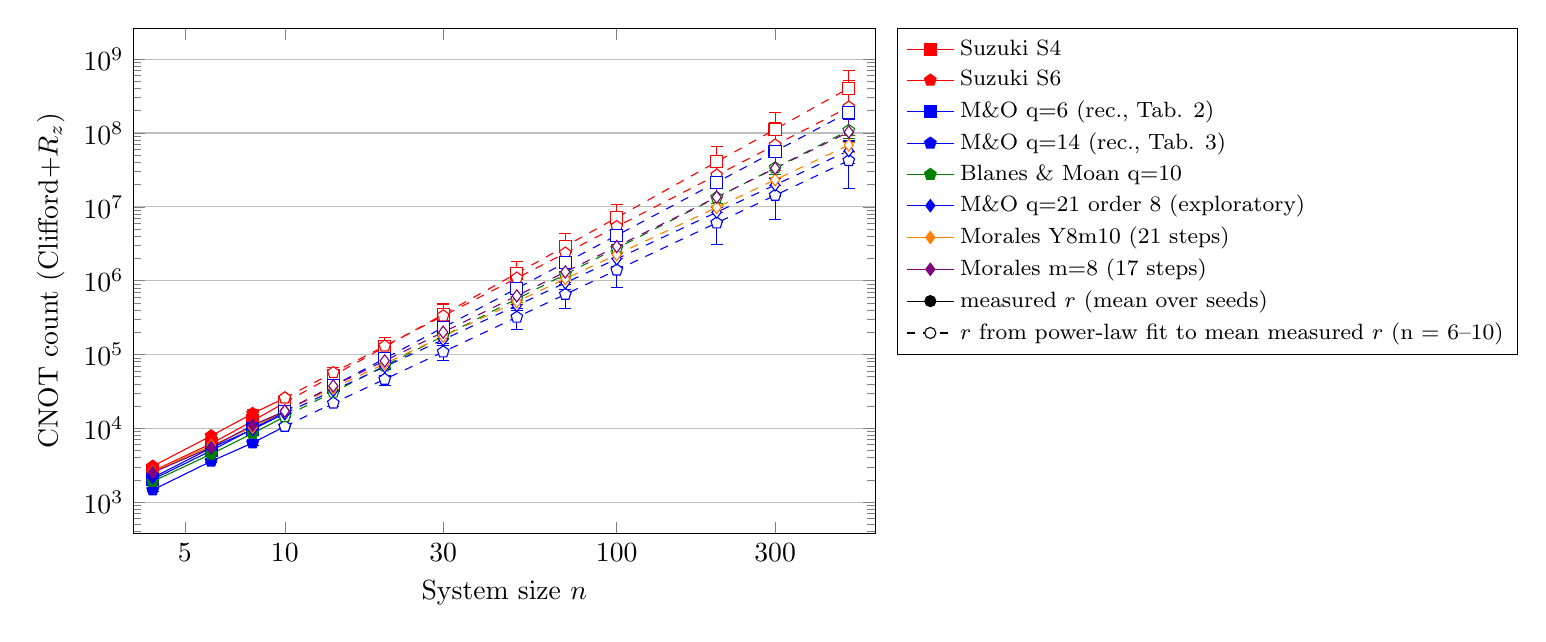
\begin{tikzpicture}
  \begin{loglogaxis}[
    width=11cm, height=8cm,
    xlabel={System size $n$},
    ylabel={CNOT count (Clifford+$R_z$)},
    xtick={5,10,30,100,300}, xticklabels={5,10,30,100,300},
    xmin=3.5, xmax=600,
    ymajorgrids=true,
    legend pos=outer north east,
    legend cell align=left,
    legend style={font=\footnotesize},
  ]
    % suzuki4: measured n, mean over seeds, bars min..max over seeds
    \addplot[red, solid, mark=square*, mark size=2.2pt, mark options={solid, fill=red}, error bars/.cd, y dir=both, y explicit, error bar style={solid}] coordinates {
      (4,2633.4) += (0,72.6) -= (0,59.4)
      (6,6177.6) += (0,59.4) -= (0,39.6)
      (8,12540) += (0,132) -= (0,132)
      (10,22275) += (0,495) -= (0,165)
    };
    \addlegendentry{Suzuki S4}
    % suzuki4: extrapolated, r = ceil(4.16533 n^1.50837), per step = 33/2 n + 0; bars min..max of per-seed fits
    \addplot[red, dashed, mark=square*, mark size=2.2pt, mark options={solid, fill=white}, forget plot, error bars/.cd, y dir=both, y explicit, error bar style={solid}] coordinates {
      (10,22275)
      (14,51744) += (0,1848) -= (0,1155)
      (20,126390) += (0,6930) -= (0,3960)
      (30,348975) += (0,28215) -= (0,15345)
      (50,1.25565e+06) += (0,139425) -= (0,74250)
      (70,2.91984e+06) += (0,384615) -= (0,203280)
      (100,7.14285e+06) += (0,1.09725e+06) -= (0,575850)
      (200,4.06428e+07) += (0,8.0289e+06) -= (0,4.1316e+06)
      (300,1.12375e+08) += (0,2.51856e+07) -= (0,1.2771e+07)
      (500,4.04712e+08) += (0,1.04569e+08) -= (0,5.20492e+07)
    };
    % suzuki6: measured n, mean over seeds, bars min..max over seeds
    \addplot[red, solid, mark=pentagon*, mark size=2.2pt, mark options={solid, fill=red}, error bars/.cd, y dir=both, y explicit, error bar style={solid}] coordinates {
      (4,3060) += (0,0) -= (0,0)
      (6,7894.8) += (0,367.2) -= (0,550.8)
      (8,15850.8) += (0,1897.2) -= (0,1774.8)
      (10,25704) += (0,1836) -= (0,1224)
    };
    \addlegendentry{Suzuki S6}
    % suzuki6: extrapolated, r = ceil(1.64221 n^1.31614), per step = 153/2 n + 0; bars min..max of per-seed fits
    \addplot[red, dashed, mark=pentagon*, mark size=2.2pt, mark options={solid, fill=white}, forget plot, error bars/.cd, y dir=both, y explicit, error bar style={solid}] coordinates {
      (10,25704)
      (14,56763) += (0,10710) -= (0,7497)
      (20,130050) += (0,38250) -= (0,26010)
      (30,332775) += (0,149175) -= (0,89505)
      (50,1.08248e+06) += (0,722925) -= (0,367200)
      (70,2.36156e+06) += (0,1.95993e+06) -= (0,904995)
      (100,5.39325e+06) += (0,5.4927e+06) -= (0,2.30265e+06)
      (200,2.68362e+07) += (0,3.88161e+07) -= (0,1.34793e+07)
      (300,6.86205e+07) += (0,1.19179e+08) -= (0,3.7156e+07)
      (500,2.2403e+08) += (0,4.81874e+08) -= (0,1.31427e+08)
    };
    % mo-q6: measured n, mean over seeds, bars min..max over seeds
    \addplot[blue, solid, mark=square*, mark size=2.2pt, mark options={solid, fill=blue}, error bars/.cd, y dir=both, y explicit, error bar style={solid}] coordinates {
      (4,2028) += (0,0) -= (0,0)
      (6,4972.5) += (0,58.5) -= (0,58.5)
      (8,9812.4) += (0,15.6) -= (0,140.4)
      (10,16848) += (0,117) -= (0,273)
    };
    \addlegendentry{M\&O q=6 (rec., Tab. 2)}
    % mo-q6: extrapolated, r = ceil(3.52884 n^1.38766), per step = 39/2 n + 0; bars min..max of per-seed fits
    \addplot[blue, dashed, mark=square*, mark size=2.2pt, mark options={solid, fill=white}, forget plot, error bars/.cd, y dir=both, y explicit, error bar style={solid}] coordinates {
      (10,16848)
      (14,37674) += (0,819) -= (0,1092)
      (20,88140) += (0,3120) -= (0,4290)
      (30,231660) += (0,11700) -= (0,16380)
      (50,783900) += (0,55575) -= (0,75075)
      (70,1.7513e+06) += (0,146055) -= (0,196560)
      (100,4.1028e+06) += (0,401700) -= (0,530400)
      (200,2.14695e+07) += (0,2.7222e+06) -= (0,3.4632e+06)
      (300,5.65227e+07) += (0,8.1315e+06) -= (0,1.0138e+07)
      (500,1.91383e+08) += (0,3.1746e+07) -= (0,3.86002e+07)
    };
    % mo-q14: measured n, mean over seeds, bars min..max over seeds
    \addplot[blue, solid, mark=pentagon*, mark size=2.2pt, mark options={solid, fill=blue}, error bars/.cd, y dir=both, y explicit, error bar style={solid}] coordinates {
      (4,1461.6) += (0,104.4) -= (0,69.6)
      (6,3575.7) += (0,339.3) -= (0,182.7)
      (8,6333.6) += (0,626.4) -= (0,417.6)
      (10,10614) += (0,261) -= (0,174)
    };
    \addlegendentry{M\&O q=14 (rec., Tab. 3)}
    % mo-q14: extrapolated, r = ceil(1.80948 n^1.12318), per step = 87/2 n + 0; bars min..max of per-seed fits
    \addplot[blue, dashed, mark=pentagon*, mark size=2.2pt, mark options={solid, fill=white}, forget plot, error bars/.cd, y dir=both, y explicit, error bar style={solid}] coordinates {
      (10,10614)
      (14,21924) += (0,1218) -= (0,2436)
      (20,46110) += (0,6090) -= (0,7830)
      (30,108315) += (0,22185) -= (0,24795)
      (50,319725) += (0,95700) -= (0,100050)
      (70,651630) += (0,243600) -= (0,237510)
      (100,1.392e+06) += (0,617700) -= (0,574200)
      (200,6.0552e+06) += (0,3.654e+06) -= (0,2.9928e+06)
      (300,1.43028e+07) += (0,1.00876e+07) -= (0,7.66035e+06)
      (500,4.23255e+07) += (0,3.55612e+07) -= (0,2.47515e+07)
    };
    % bm-q10: measured n, mean over seeds, bars min..max over seeds
    \addplot[green!50!black, solid, mark=pentagon*, mark size=2.2pt, mark options={solid, fill=green!50!black}, error bars/.cd, y dir=both, y explicit, error bar style={solid}] coordinates {
      (4,1902.6) += (0,113.4) -= (0,12.6)
      (6,4479.3) += (0,56.7) -= (0,132.3)
      (8,8517.6) += (0,50.4) -= (0,201.6)
      (10,14395.5) += (0,409.5) -= (0,220.5)
    };
    \addlegendentry{Blanes \& Moan q=10}
    % bm-q10: extrapolated, r = ceil(2.3688 n^1.28299), per step = 63/2 n + 0; bars min..max of per-seed fits
    \addplot[green!50!black, dashed, mark=pentagon*, mark size=2.2pt, mark options={solid, fill=white}, forget plot, error bars/.cd, y dir=both, y explicit, error bar style={solid}] coordinates {
      (10,14395.5)
      (14,30870) += (0,2205) -= (0,882)
      (20,69930) += (0,8190) -= (0,4410)
      (30,176715) += (0,29295) -= (0,15120)
      (50,565425) += (0,133875) -= (0,63000)
      (70,1.21716e+06) += (0,348390) -= (0,154350)
      (100,2.7468e+06) += (0,932400) -= (0,396900)
      (200,1.33686e+07) += (0,6.0102e+06) -= (0,2.394e+06)
      (300,3.37365e+07) += (0,1.74825e+07) -= (0,6.6906e+06)
      (500,1.08281e+08) += (0,6.5961e+07) -= (0,2.40345e+07)
    };
    % mo-o8-q21: measured n, mean over seeds, bars min..max over seeds
    \addplot[blue, solid, mark=diamond*, mark size=2.2pt, mark options={solid, fill=blue}, error bars/.cd, y dir=both, y explicit, error bar style={solid}] coordinates {
      (4,2141.4) += (0,180.6) -= (0,77.4)
      (6,5418) += (0,387) -= (0,387)
      (8,9649.2) += (0,670.8) -= (0,361.2)
      (10,15867) += (0,903) -= (0,387)
    };
    \addlegendentry{M\&O q=21 order 8 (exploratory)}
    % mo-o8-q21: extrapolated, r = ceil(1.93865 n^1.0989), per step = 129/2 n + 0; bars min..max of per-seed fits
    \addplot[blue, dashed, mark=diamond*, mark size=2.2pt, mark options={solid, fill=white}, forget plot, error bars/.cd, y dir=both, y explicit, error bar style={solid}] coordinates {
      (10,15867)
      (14,32508) += (0,2709) -= (0,1806)
      (20,68370) += (0,9030) -= (0,5160)
      (30,158670) += (0,34830) -= (0,17415)
      (50,461175) += (0,154800) -= (0,70950)
      (70,934605) += (0,392805) -= (0,171570)
      (100,1.9737e+06) += (0,1.0062e+06) -= (0,419250)
      (200,8.4495e+06) += (0,5.9469e+06) -= (0,2.2704e+06)
      (300,1.9795e+07) += (0,1.63701e+07) -= (0,5.94045e+06)
      (500,5.78242e+07) += (0,5.7663e+07) -= (0,1.95435e+07)
    };
    % morales-y8m10: measured n, mean over seeds, bars min..max over seeds
    \addplot[orange, solid, mark=diamond*, mark size=2.2pt, mark options={solid, fill=orange}, error bars/.cd, y dir=both, y explicit, error bar style={solid}] coordinates {
      (4,2580) += (0,0) -= (0,0)
      (6,5805) += (0,0) -= (0,0)
      (8,10320) += (0,0) -= (0,0)
      (10,17221.5) += (0,193.5) -= (0,451.5)
    };
    \addlegendentry{Morales Y8m10 (21 steps)}
    % morales-y8m10: extrapolated, r = ceil(1.98514 n^1.12271), per step = 129/2 n + 0; bars min..max of per-seed fits
    \addplot[orange, dashed, mark=diamond*, mark size=2.2pt, mark options={solid, fill=white}, forget plot, error bars/.cd, y dir=both, y explicit, error bar style={solid}] coordinates {
      (10,17221.5)
      (14,35217) += (0,903) -= (0,903)
      (20,74820) += (0,1290) -= (0,3870)
      (30,176085) += (0,5805) -= (0,13545)
      (50,519225) += (0,22575) -= (0,48375)
      (70,1.06102e+06) += (0,49665) -= (0,117390)
      (100,2.2575e+06) += (0,129000) -= (0,283800)
      (200,9.8169e+06) += (0,722400) -= (0,1.5222e+06)
      (300,2.322e+07) += (0,1.91565e+06) -= (0,4.00545e+06)
      (500,6.8628e+07) += (0,6.5145e+06) -= (0,1.32548e+07)
    };
    % morales-m8: measured n, mean over seeds, bars min..max over seeds
    \addplot[violet, solid, mark=diamond*, mark size=2.2pt, mark options={solid, fill=violet}, error bars/.cd, y dir=both, y explicit, error bar style={solid}] coordinates {
      (4,2520) += (0,0) -= (0,0)
      (6,5512.5) += (0,157.5) -= (0,157.5)
      (8,11004) += (0,336) -= (0,504)
      (10,17062.5) += (0,787.5) -= (0,787.5)
    };
    \addlegendentry{Morales m=8 (17 steps)}
    % morales-m8: extrapolated, r = ceil(1.995 n^1.22085), per step = 105/2 n + 0; bars min..max of per-seed fits
    \addplot[violet, dashed, mark=diamond*, mark size=2.2pt, mark options={solid, fill=white}, forget plot, error bars/.cd, y dir=both, y explicit, error bar style={solid}] coordinates {
      (10,17062.5)
      (14,37485) += (0,2940) -= (0,3675)
      (20,81900) += (0,11550) -= (0,11550)
      (30,200025) += (0,42525) -= (0,36225)
      (50,622125) += (0,189000) -= (0,152250)
      (70,1.31198e+06) += (0,485100) -= (0,367500)
      (100,2.898e+06) += (0,1.2705e+06) -= (0,918750)
      (200,1.3503e+07) += (0,7.9275e+06) -= (0,5.1765e+06)
      (300,3.32325e+07) += (0,2.26328e+07) -= (0,1.3923e+07)
      (500,1.0332e+08) += (0,8.34225e+07) -= (0,4.76438e+07)
    };
    \addlegendimage{black, solid, mark=*, mark options={solid, fill=black}}
    \addlegendentry{measured $r$ (mean over seeds)}
    \addlegendimage{black, dashed, mark=*, mark options={solid, fill=white}}
    \addlegendentry{$r$ from power-law fit to mean measured $r$ (n = 6--10)}
  \end{loglogaxis}
\end{tikzpicture}
